% This file was created by matplotlib2tikz v0.6.16.
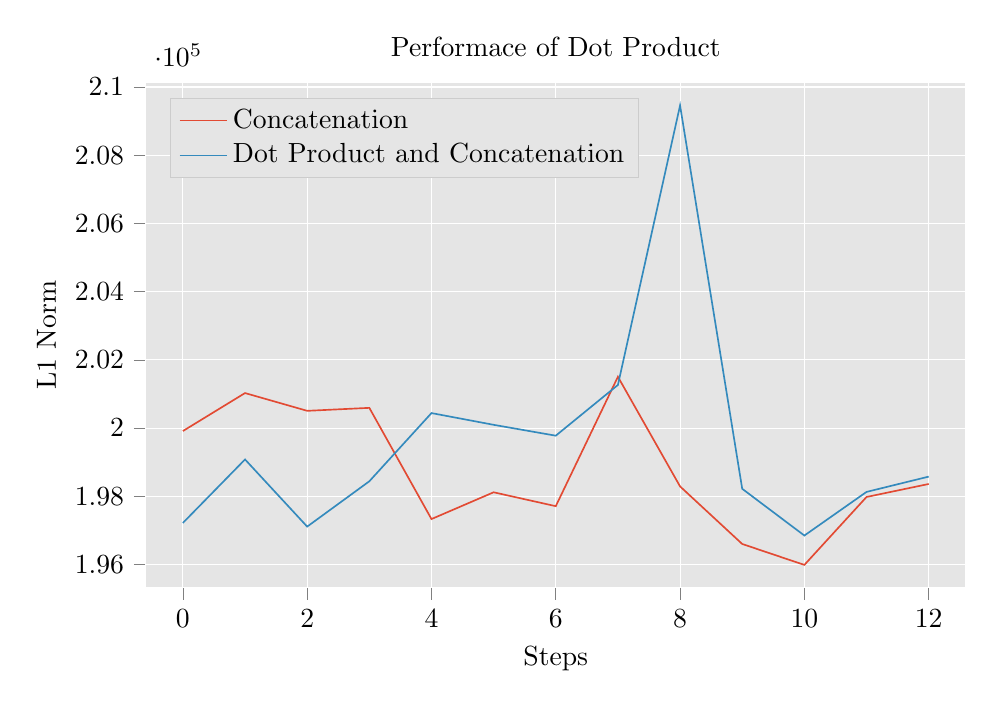
\begin{tikzpicture}

\definecolor{color1}{rgb}{0.203921568627451,0.541176470588235,0.741176470588235}
\definecolor{color0}{rgb}{0.886274509803922,0.290196078431373,0.2}

\begin{axis}[
title={Performace of Dot Product},
xlabel={Steps},
ylabel={L1 Norm},
xmin=-0.6, xmax=12.6,
ymin=195314.278125, ymax=210133.065625,
width=12cm,
height=8cm,
tick align=outside,
tick pos=left,
xmajorgrids,
x grid style={white},
ymajorgrids,
y grid style={white},
axis line style={white},
axis background/.style={fill=white!89.80392156862746!black},
legend style={at={(0.03,0.97)}, anchor=north west, draw=white!80.0!black, fill=white!89.80392156862746!black},
legend entries={{Concatenation},{Dot Product and Concatenation}},
legend cell align={left}
]
\addlegendimage{no markers, color0}
\addlegendimage{no markers, color1}
\addplot [semithick, color0]
table {%
0 199912.765625
1 201026.984375
2 200505.734375
3 200593.0625
4 197332.296875
5 198117.484375
6 197710.078125
7 201504.21875
8 198289.265625
9 196601.453125
10 195987.859375
11 197979.546875
12 198360.421875
};
\addplot [semithick, color1]
table {%
0 197218.3125
1 199080.0625
2 197110.71875
3 198440.03125
4 200439.765625
5 200095.78125
6 199776.78125
7 201264.515625
8 209459.484375
9 198219.90625
10 196848.78125
11 198128.296875
12 198576.578125
};
\end{axis}

\end{tikzpicture}